\chapter*{Задание 1}
Процессы-сироты. В программе создаются не менее двух потомков. В потомках вызывается sleep(). 
Чтобы предок гарантированно завершился раньше своих потомков. 
Продемонстрировать с помощью соответствующего вывода информацию об идентификаторах процессов и их группе. 
Продемонстрировать «усыновление». 
Для этого надо в потомках вывести идентификаторы: собственный, предка, группы до блокировки и после блокировки.

На листинге 1 представлен код программы:
\FloatBarrier
\begin{lstinputlisting}[language=C++, caption=Код задания 1, 
	linerange={1-37}, basicstyle=\footnotesize\ttfamily, showstringspaces=false, frame=single,breaklines=true]{src/1.c}
\end{lstinputlisting}
\FloatBarrier

На рисунке 1 продемонстрирован вывод программы:
\FloatBarrier
\begin{figure}[h]
	\begin{center}
		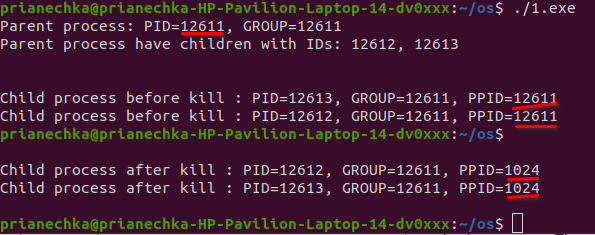
\includegraphics[]{inc/first.png}
	\end{center}
	\caption{Демонстрация работы программы}
\end{figure}
\FloatBarrier

Лабораторная выполнялась на Ubuntu.
Как видно, идентификатор предка для потомков действительно сменился на идентификатора процесса-посредника.

\chapter*{Задание 2}
Предок ждет завершения своих потомком, используя системный вызов wait(). 
Вывод соответствующих сообщений на экран. 
В программе необходимо, чтобы предок выполнял анализ кодов завершения потомков.

На листинге 2 представлен код программы:
\FloatBarrier
\begin{lstinputlisting}[language=C++, caption=Код задания 2, 
	linerange={1-60}, basicstyle=\footnotesize\ttfamily, showstringspaces=false, frame=single,breaklines=true]{src/2.c}
\end{lstinputlisting}
\FloatBarrier


На рисунке 2 продемонстрирован вывод программы:
\FloatBarrier
\begin{figure}[h]
	\begin{center}
		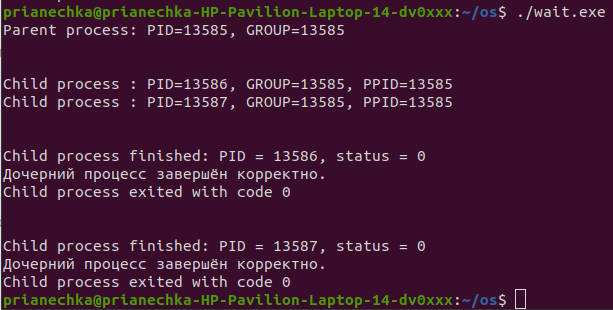
\includegraphics[]{inc/second.png}
	\end{center}
	\caption{Демонстрация работы программы}
\end{figure}
\FloatBarrier

Видно, что сначала завершились все потомки, а только затем -- предок.

\chapter*{Задание 3}
Потомки переходят на выполнение других программ, которые передаются системному вызову exec() в качестве параметра. 
Потомки должны выполнять разные программы. 
Предок ждет завершения своих потомков с анализом кодов завершения. 
На экран выводятся соответствующие сообщения.

На листинге 3 представлен код программы:

\FloatBarrier
\begin{lstinputlisting}[language=C++, caption=Код задания 3, 
	linerange={1-84}, basicstyle=\footnotesize\ttfamily, showstringspaces=false, frame=single,breaklines=true]{src/3.c}
\end{lstinputlisting}
\FloatBarrier

В качестве программ, которые вызываются программой exec выбраны:
\begin{enumerate}
	\item Быстрая сортировка массива;
	\item Программа вычисления наиболее коррелирующих столбцов матрицы при помощи поточных вычислений (из курса "Анализ Алгоритмов")
\end{enumerate}

На рисунке 3 продемонстрирован вывод программы:
\FloatBarrier
\begin{figure}[h]
	\begin{center}
		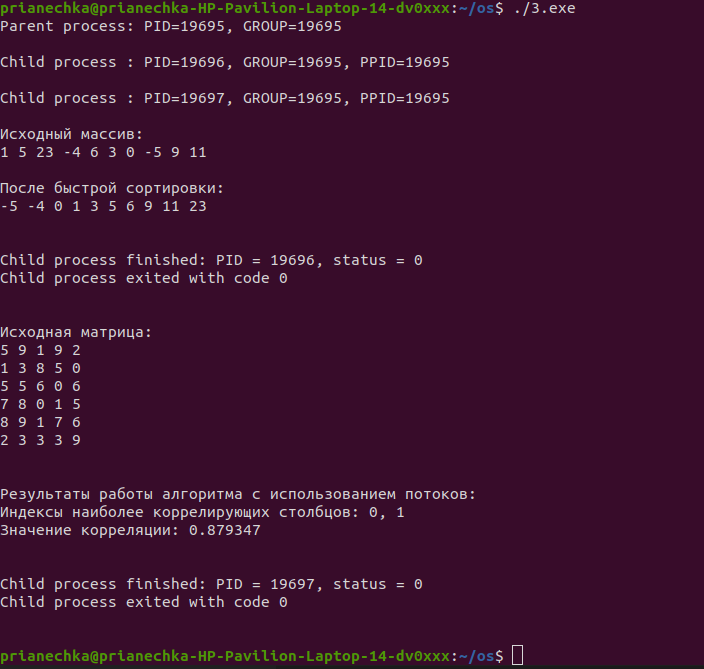
\includegraphics[]{inc/third.png}
	\end{center}
	\caption{Демонстрация работы программы}
\end{figure}
\FloatBarrier

Также в этом задании была смоделирована ситуация, когда дочерний процесс не был корректно завершён:
\FloatBarrier
\begin{figure}[h]
	\begin{center}
		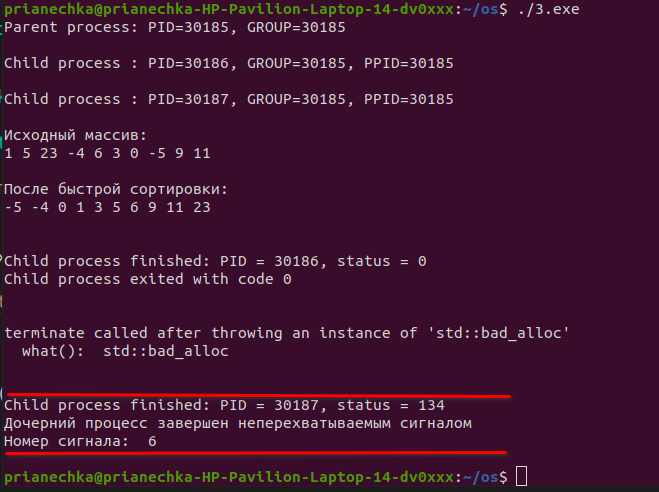
\includegraphics[]{inc/error.png}
	\end{center}
	\caption{Демонстрация работы программы}
\end{figure}
\FloatBarrier

\chapter*{Задание 4}
Предок и потомки обмениваются сообщениями через неименованный программный канал. 
Причем оба потомка пишут свои сообщения в один программный канал, а предок их считывает из канала. 
Потомки должны посылать предку разные сообщения по содержанию и размеру. 
Предок считывает сообщения от потомков и выводит их на экран. 
Предок ждет завершения своих потомков и анализирует код их завершения. 
Вывод соответствующих сообщений на экран.

На листинге 4 представлен код программы:
\FloatBarrier
\begin{lstinputlisting}[language=C++, caption=Код задания 4, 
	linerange={1-76}, basicstyle=\footnotesize\ttfamily, showstringspaces=false, frame=single,breaklines=true]{src/4.c}
\end{lstinputlisting}
\FloatBarrier

На рисунке 5 продемонстрирован вывод программы:
\FloatBarrier
\begin{figure}[h]
	\begin{center}
		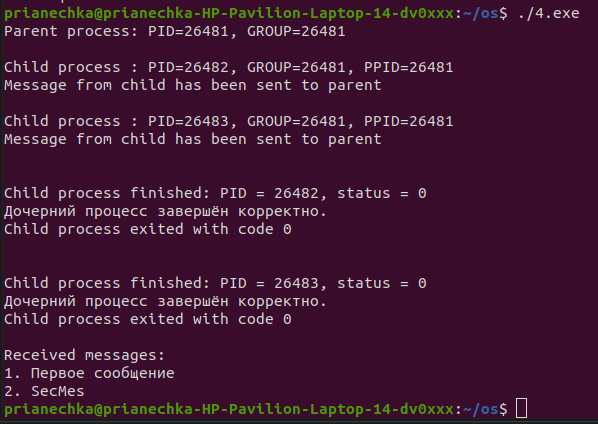
\includegraphics[]{inc/forth.png}
	\end{center}
	\caption{Демонстрация работы программы}
\end{figure}
\FloatBarrier

\chapter*{Задание 5}
Предок и потомки аналогично п.4 обмениваются сообщениями через неименованный программный канал. 
В программу включается собственный обработчик сигнала. 
С помощью сигнала меняется ход выполнения программы. 
При получении сигнала потомки записывают сообщения в канал, если сигнал не поступает, то не записывают. 
Предок ждет завершения своих потомков и анализирует коды их завершений. 
Вывод соответствующих сообщений на экран.

На листинге 5 представлен код программы:

\FloatBarrier
\begin{lstinputlisting}[language=C++, caption=Код задания 5, 
	linerange={1-92}, showstringspaces=false, basicstyle=\footnotesize\ttfamily, frame=single,breaklines=true]{src/5.c}
\end{lstinputlisting}
\FloatBarrier

На рисунке 6 продемонстрирован вывод программы в случае получения сигнала:

\FloatBarrier
\begin{figure}[h]
	\begin{center}
		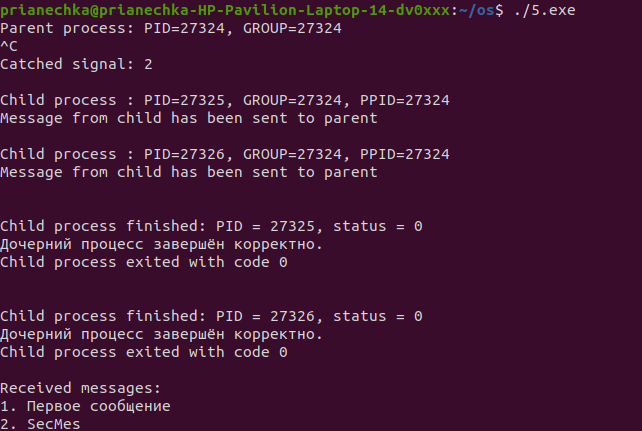
\includegraphics[]{inc/five_yes.png}
	\end{center}
	\caption{Демонстрация работы программы}
\end{figure}
\FloatBarrier

На рисунке 7 продемонстрирован вывод программы в случае не получения сигнала:

\FloatBarrier
\begin{figure}[h]
	\begin{center}
		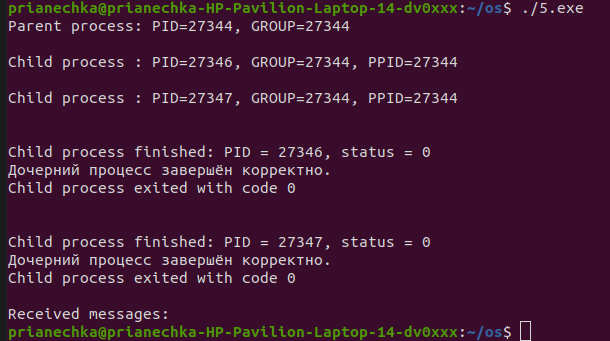
\includegraphics[]{inc/five_no.png}
	\end{center}
	\caption{Демонстрация работы программы}
\end{figure}
\FloatBarrier

\chapter*{Конспект}

\FloatBarrier
\begin{figure}[h]
	\begin{center}
		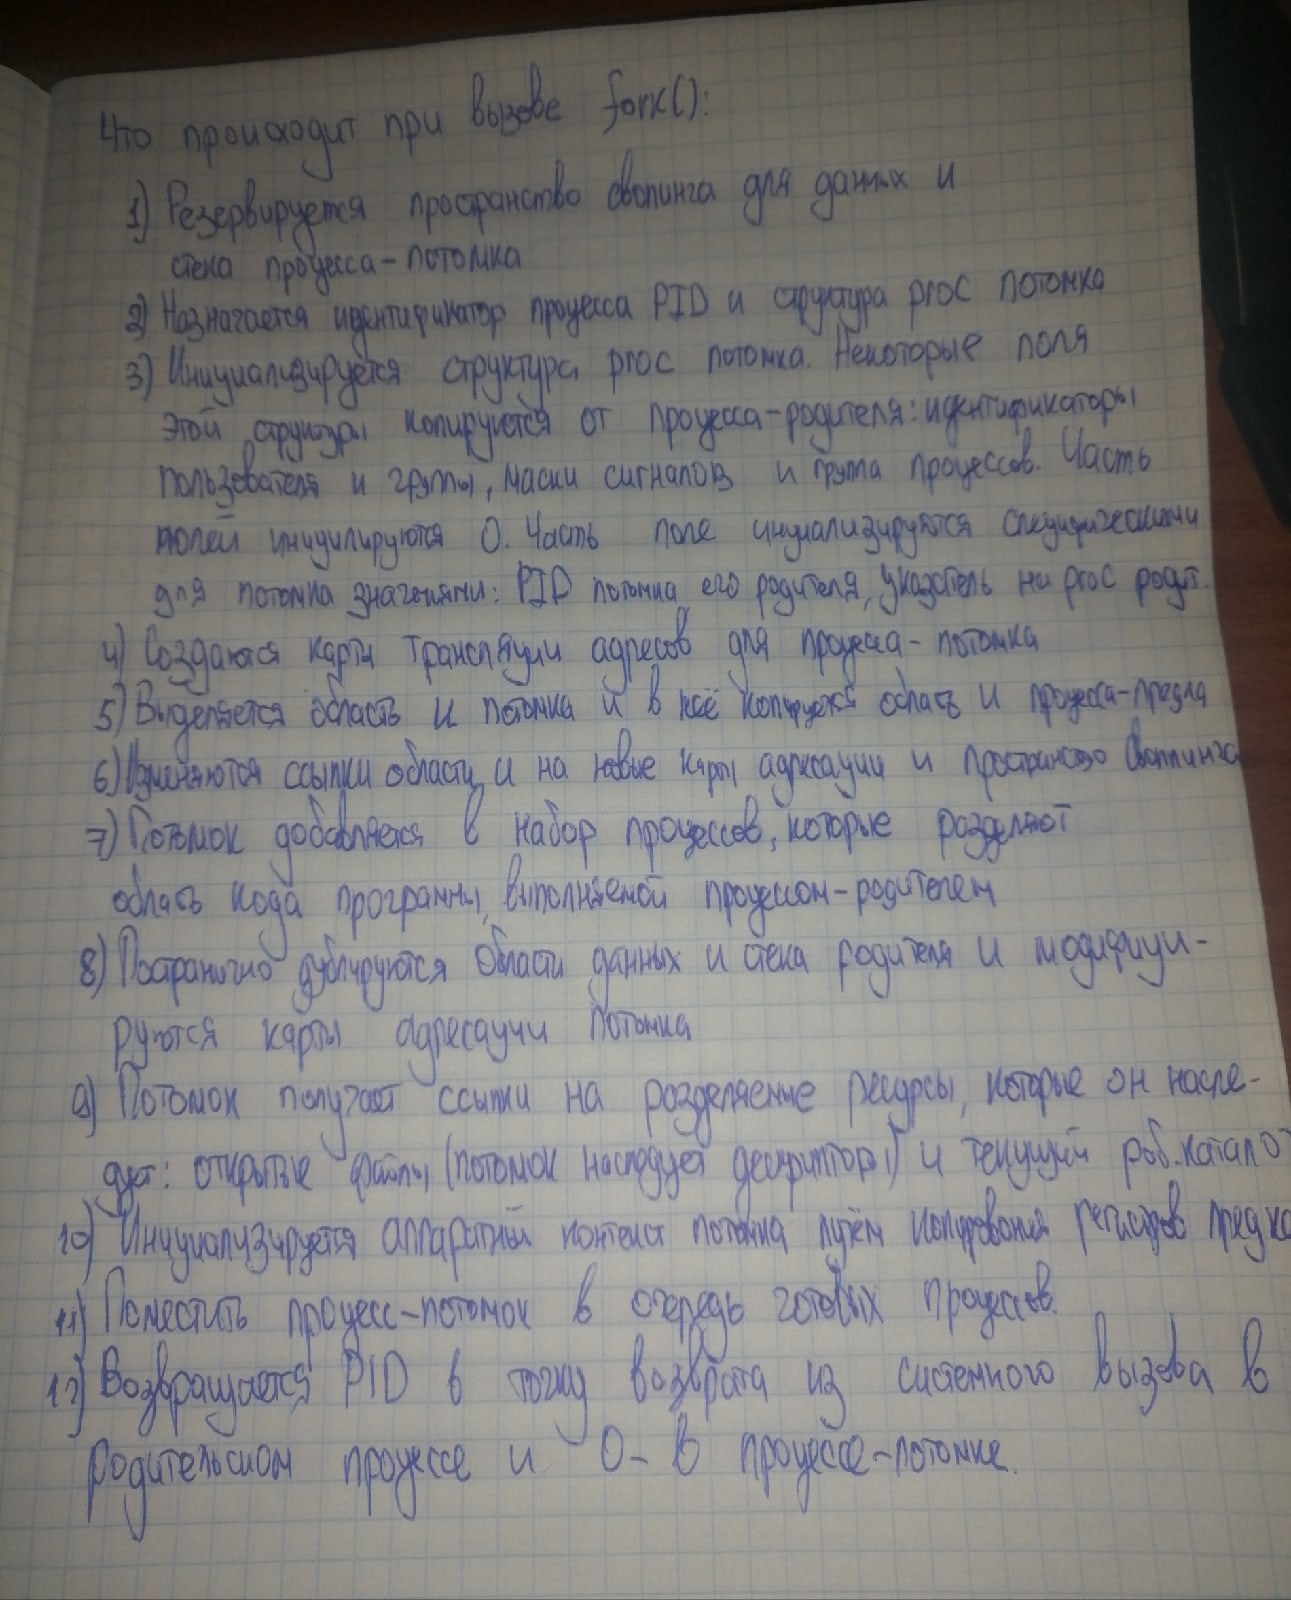
\includegraphics[width = \linewidth, height = 17cm ]{inc/fork.jpg}
	\end{center}
	\caption{Конспект по fork}
\end{figure}
\FloatBarrier

\FloatBarrier
\begin{figure}[h]
	\begin{center}
		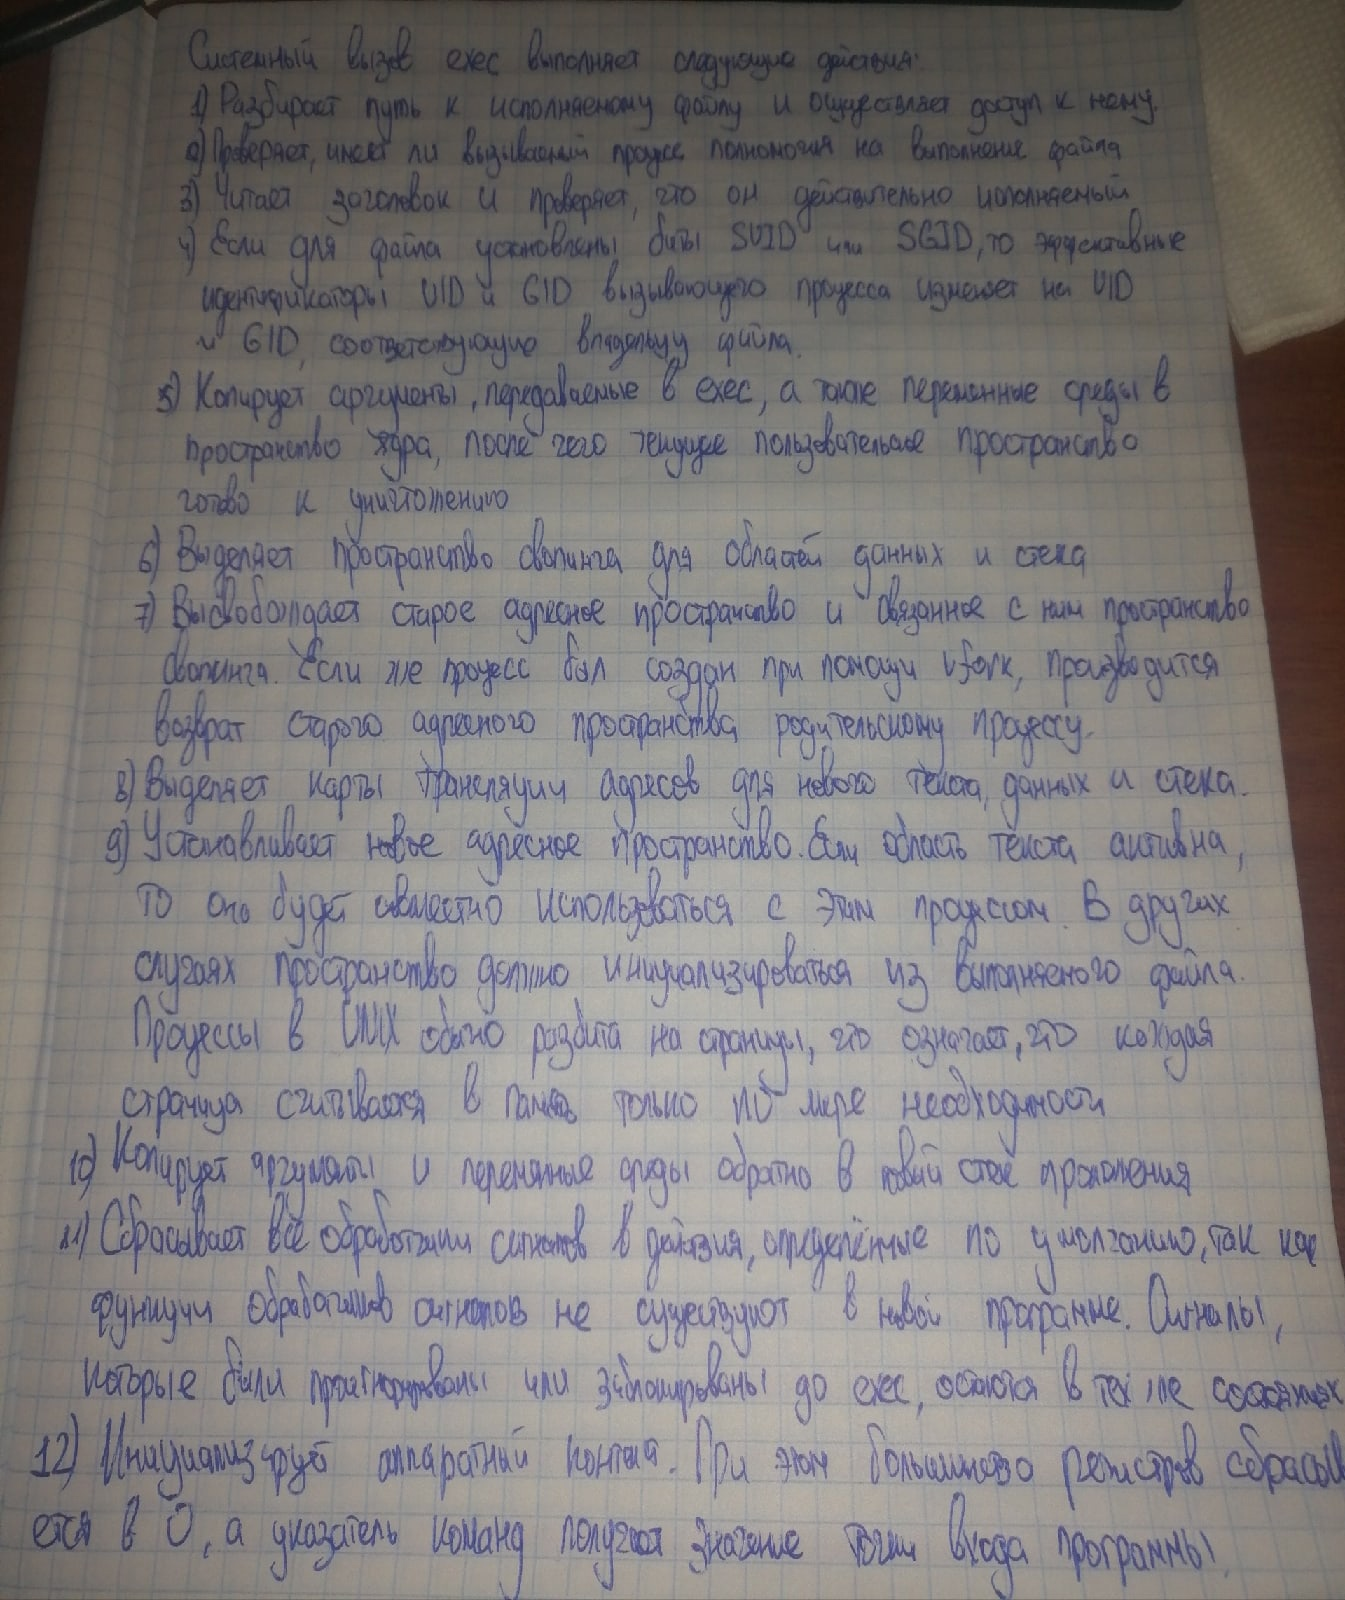
\includegraphics[width = \linewidth]{inc/exec.jpg}
	\end{center}
	\caption{Конспект по exec}
\end{figure}
\FloatBarrier